\documentclass{standalone}
\usepackage{graphicx}	
\usepackage{amssymb, amsmath}
\usepackage{color}

\usepackage{tikz}
\usetikzlibrary{shapes}
\usepackage{pgfmath}

\definecolor{light}{RGB}{220, 188, 188}
\definecolor{mid}{RGB}{185, 124, 124}
\definecolor{dark}{RGB}{143, 39, 39}
\definecolor{highlight}{RGB}{180, 31, 180}
\definecolor{lightteal}{RGB}{107, 142, 142}
\definecolor{midteal}{RGB}{72, 117, 117}
\definecolor{darkteal}{RGB}{29, 79, 79}
\definecolor{gray10}{gray}{0.1}
\definecolor{gray20}{gray}{0.2}
\definecolor{gray30}{gray}{0.3}
\definecolor{gray40}{gray}{0.4}
\definecolor{gray60}{gray}{0.6}
\definecolor{gray70}{gray}{0.7}
\definecolor{gray80}{gray}{0.8}
\definecolor{gray90}{gray}{0.9}
\definecolor{gray95}{gray}{0.95}

\newcommand*{\offset}{0.025}

\begin{document}

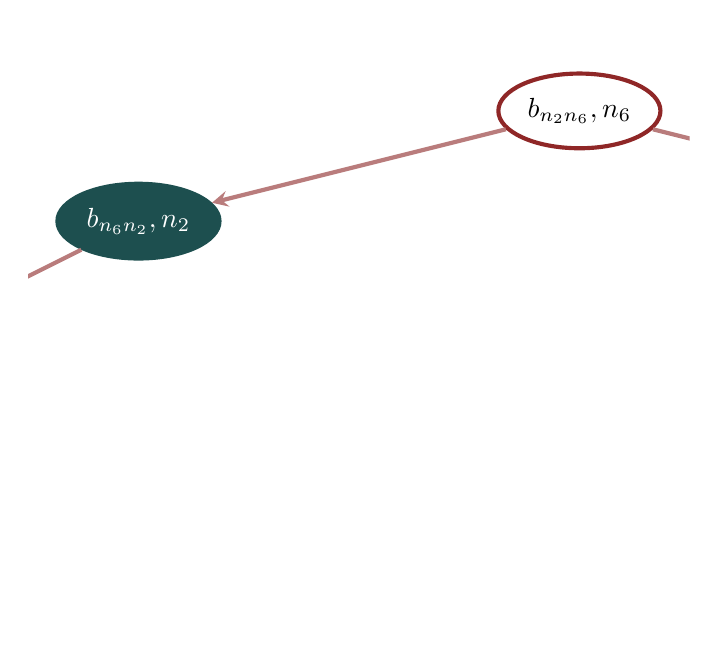
\begin{tikzpicture}[
   scale=0.2,
   obscirc/.style={circle, draw=dark, fill=dark, line width=1.5, text=white,
               inner sep=5, minimum size=27},
   obsell/.style={ellipse, draw=dark, fill=dark, line width=1.5, text=white,
                  inner sep=5, minimum height=27},
   nell/.style={ellipse, draw=darkteal, fill=darkteal, line width=1.5, text=white,
                  inner sep=2, minimum height=27},
   unobscirc/.style={circle, draw=dark, fill=white, line width=1.5, text=black,
                     inner sep=5, minimum size=27},
   unobsell/.style={ellipse, draw=dark, fill=white, line width=1.5, text=black,
                    inner sep=2, minimum height=27}
  ]

  % Node Spacing
  \pgfmathsetmacro{\d}{7}
  
  \begin{scope}[shift={(0, 0)}]
    \draw[white] (-5 * \d, -4.75 * \d) rectangle (1 * \d, 0.75 * \d);
    \clip (-5 * \d, -4.75 * \d) rectangle (1 * \d, 0.75 * \d);
  
    \node (N1) at (0 * \d, 0 * \d) [unobsell] { $b_{n_{2} n_{6}}, n_{6}$ };
    
    \node (N2) at (-4 * \d, -1 * \d) [nell] { $b_{n_{6} n_{2}}, n_{2}$ };
    \node (N3) at (+4 * \d, -1 * \d) {};

    %\node (N4) at (-2 * \d, -2 * \d) [unobscirc] { $n_{2}$ };
    \node (N5) at (-6 * \d, -2 * \d) {};

    \foreach \B/\E in {N1/N2, N1/N3, N2/N5} {
      \draw[->, >=stealth, color=mid, line width=1.5] (\B) -- (\E);
    }
    
    %\node (N6) at (-2 * \d, -2 * \d) [unobsell] { $b_{n_{2} n_{9}}, n_{9}$ };
    %\node (N8) at (-1 * \d, -3 * \d) [unobsell] { $b_{n_{9} n_{2}}, n_{2}$ };

    \foreach \B/\E in {} {
      \draw[->, >=stealth, color=mid, line width=1.5] (\B) -- (\E);
    }

  \end{scope}

\end{tikzpicture}

\end{document}  